\documentclass{article}
\usepackage {graphicx}
\usepackage{listings}


\title{Instagram Fake Users Recognition with different Classification Techniques}
\date{26/02/2020}
\author{Fernando De Nitto\\Francesco Fornaini\\\\\ Data Mining Course\\ Department of Information Engineering\\ University of Pisa\\}
 
 
\begin{document}

\maketitle


\section{The Goal of Project}
Scrivere cosa volevamo raggiungere con questo progetto del cazzo dio cane

 \begin{figure}[!h]
 \center
  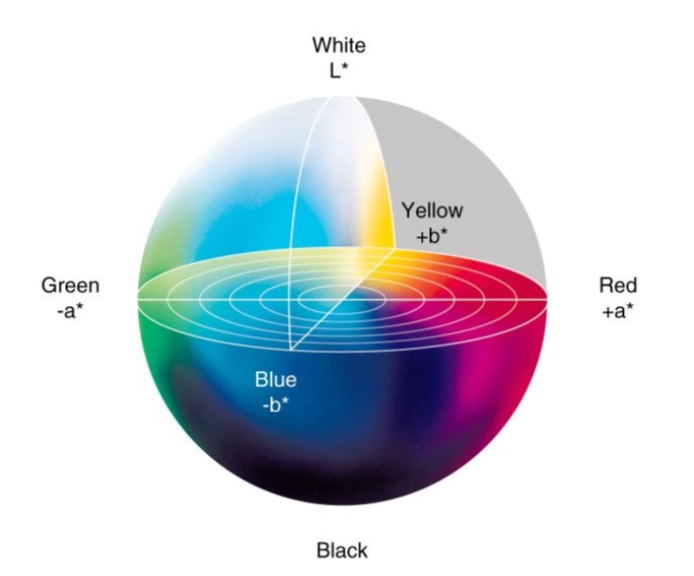
\includegraphics[width=170pt]{img/cielab.jpg}
  \caption{CIE Lab Color Space}
  \label{fig:cielab}
\end{figure}

\section{Problems and Challenges}
In this section we want to discuss why spend efforts on Instagram Social Network and which challenges are linked with this kind of Social Network. All the considerations could be extend in every social network that follows the pattern of Instagram.

\subsection{Instagram}
Scrivere cosa vogliamo fare

\section{Dataset}
Scrivere cosa vogliamo fare


\section{Classification}
Scrivere cosa vogliamo fare

\subsection{SVM}
Scrivere cosa vogliamo fare

\subsection{KNN}
Scrivere cosa vogliamo fare

\subsection{Multi-Layer Perceptron}
Scrivere cosa vogliamo fare

\subsection{Decision Tree}
Scrivere cosa vogliamo fare

\subsection{Random Forest}
Scrivere cosa vogliamo fare

\section{Results}
Scrivere cosa vogliamo fare

\section{Conclusion}
Scrivere cosa vogliamo fare

\end{document}



